\documentclass[11pt]{article}
\usepackage[T1]{fontenc}
\usepackage[utf8]{inputenc}
\usepackage[francais]{babel}
\usepackage[a4paper]{geometry}
\usepackage{color}
\usepackage{changepage}
\usepackage{float}

\usepackage {graphicx}
\usepackage { }

\begin{document}
\begin{figure}
    
\includegraphics[height=1cm]{logolemansU.png}
    \hfill
    
\includegraphics[height=1cm]{logo_IC2.png}
\end{figure}
    \title { 
        \textcolor{blue}{Le Mans Université} \\
        \texttt{Licence Informatique 2ème année} \\
        \texttt{Module 174UP02 Rapport de projet}\\
        \textbf{Titre du projet}
    }
    
    \author{Nathan M, Ilann T, Lucas R, Baptiste M} 
    \date{\today} 
    \maketitle
    

    \newpage
    \tableofcontents
    
    \section{Introduction}
    
    \section{Conception}

        \subsection{Cahier de charges}

        \subsection{Fonctionnalités} 
    
    \section{Organisation du Projet}
        \subsection{Planning Prévisionnel et répartition des tâches}
        Nous nous sommes répartis les tâches de la manière indiquée ci-dessous. Voir Figure ~\ref{fig:Gant}
        \begin{center}
            \begin{figure}[H]
                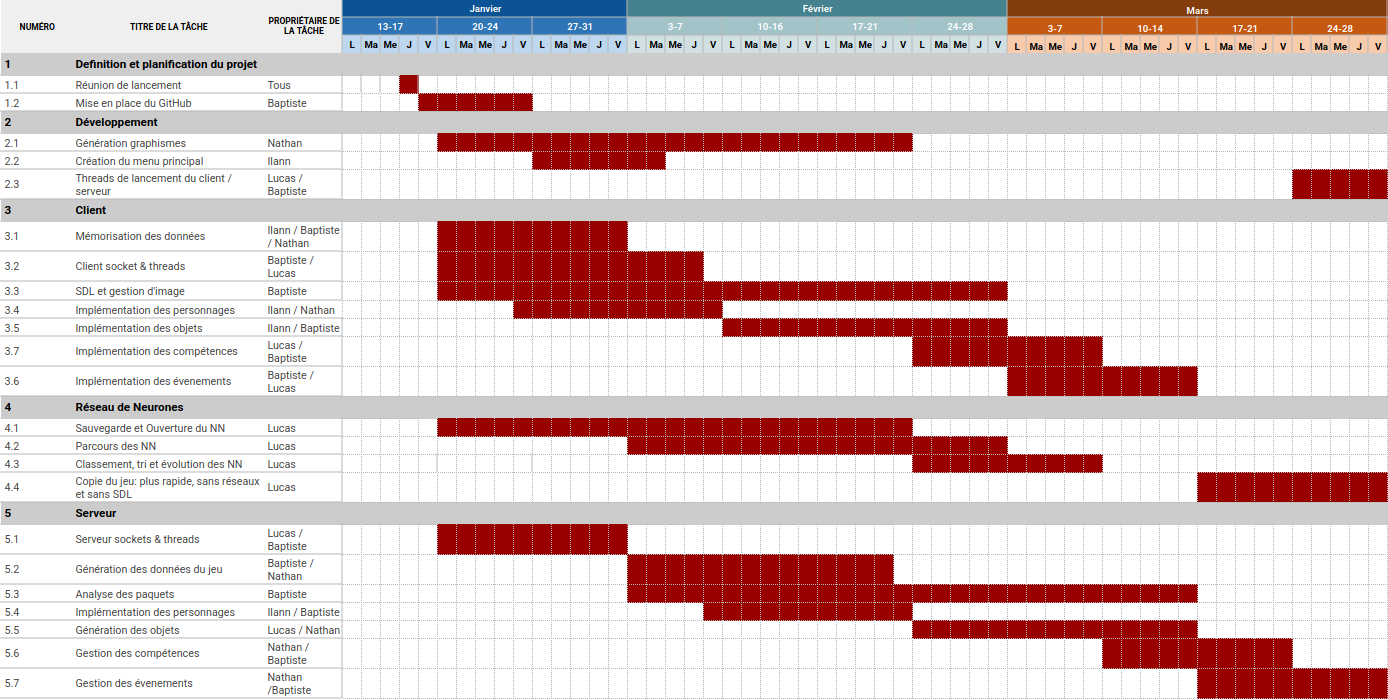
\includegraphics[height=7.3cm]{gant.png}
                \caption{Diagramme Gant}
                \label{fig:Gant}
            \end{figure}
        \end{center}
    \section{Développement}
    Cette partie abordera le développement du jeu dans sa globalité. De la création des ressources graphique à la création du client/serveur en passant par la gestion des de la carte, des objets etc. 
        \subsection{Création des ressources}
            \subsubsection{Objet}
            \subsubsection{Sprites et Personnages}
            \subsubsection{Boutons}
            \subsubsection{Sorts}
        \subsection{Implémentation}
            \subsubsection{Map}
            \subsubsection{Compétences}
            \subsubsection{Objets}
            \subsubsection{Quêtes}
            \subsubsection{Personnages non joueurs}
            Plusieurs personnages non joueurs sont présents dans le jeu. 
            Premièrement il y a les monstres, apellés mobs. Lorsqu'il sont tués il permettent d'obtenir des objets qui augmentent les capacités de base de notre personnage.
            Les mobs ont plusieurs fonctionnalités. La première est qu'ils se rapprochent du joueur le plus proche à l'aide d'une fonction de calcul de distance.
            Une fois que cette distance est calculée la direction que le mob doit prendre est choisie avec un calcul d'angle. 
            Un vecteur horizontal orienté à droite est créé ainsi qu'un vecteur personnage vers mobs. On calcule l'angle en radians formé par ces deux vecteurs.
            On obtient donc une valeur du cercle trigonométrique que l'on exploite de la manière suivante : 
            \begin{itemize}
                \item Le monstre va en haut si   pi/4 <= angle < 3pi/4
                \item Le monstre va a gauche si  3pi/4 <= angle < 5pi/4
                \item Le monstre va en bas si    5pi/4 <= angle < 7pi/4
                \item Le monstre va a droite dans tous les autres cas
            \end{itemize}
            \subsubsection{Évènement}
        \subsection{Réseau}
            \subsubsection{Client}
            \subsubsection{Serveur}
        \subsection{Rendu Graphique}
            \subsubsection{Menu Principal}
            \subsubsection{Jeu}
                \paragraph{Personnages}
                \paragraph{Environnement}
    
    \section{Résultats et conslusion}
    \section{Annexes}

\end{document}